\chapter{Implementation}
  We implemented our optimization as an addition to \textit{AutoWDS basic}, after it successfully created a stable network tree topology (See Chapter \ref{autowdsbasic}).
  The additional steps in the discovery process of nearby radios are:
  
  \begin{enumerate}
   \item The APs enable the background scan. This means the APs cycle through all possible channels for a few milliseconds 
    and listen for other broadcasted wireless networks and store the recognized mac addresses and signal strength in a corresponding table.
    Note the APs regularly switch to the background-scan-mode to discover other APs.
   \item APs send scan results continuously to the central \ac{WLC}.
   \item When all the scan results are in, we read the scan-results table from the \ac{WLC} to our client station and parse the data to a networkX graph.
   \item On the client station we compute an optimized network topology for a given set of input parameters set by the administrator. 
   \item Write back the data from the client station to the WLC to the configure-topology-table.
   \item The \ac{WLC} derives configurations in \ac{TLV}-format (\ac{CAPWAP}) and sends these to the APs.
   \item The APs receive the configurations and reconfigure themselves to establish the new network links.
   \item After a while all the APs solely use the newly configured connections and announce the network to other stations and clients.
  \end{enumerate}
  
  Later eventually steps three to five will be also incorporated in the \ac{WLC} to make the process optimization more convenient.
  
  \begin{figure}[h!]
    \centering
    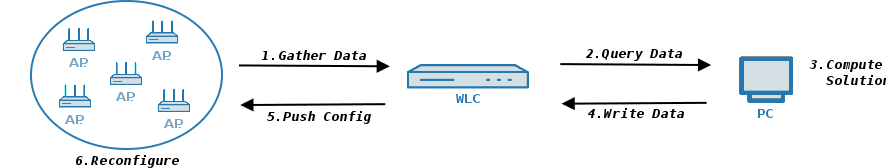
\includegraphics[width=1\columnwidth]{figures/dataflow}
    \caption{General flow of information in \textit{AutoWDS extended}}
    \label{fig:dataflow}
  \end{figure}

  \section{Language of Choice}
    The language we used for the implementation is Python 2.7.
    Although we also could have implemented the extension in c/c++ since the basic version was already written in this language,
    python does have a certain key advantages, we did not want to miss and want to list here.
    
    \begin{description}
      \item [Rapid prototyping:]
	Since our algorithms can easily work on a given set of data independently and the interfaces to get the data from are well defined and accessible,
	using a lightweight language like python had the benefit of not having to embed our new code into the existing environment. 
	Although it still can be implemented in the native language C/C++ for our scenario, this will take more time and effort, which was not the focus of this work.
      \item[Existing libraries:]
	The NetworkX library in python made it particularly easy for us to map real world scenarios to graph abstractions as we did not have to create those structures ourselves.
	Although there are some libraries that provide graph abstractions in C/C++ we could not have as easily employed them due to their copyright restrictions and 
	the closed source virtue of our target system.
      \item[Faster Debugging:]
	Especially the initial phase of the project was error-prone and needed a lot of debugging.
	Secluding our algorithm from \ac{LCOS} brought the advantage of not having to undergo the lengthy process of compiling a whole new LCOS firmware,
	every time we made a fix in our code.
	Additionally not having to flash the firmware then into the \ac{WLC} was a great time saver as keeping the \ac{WLC} running and consequently the APs connected,
	allowed us to independently modify our algorithms without having to wait until the network was back up again. 
	Not to mention the live debugging capabilities of python, which was really helpful and made debugging easy.
      \item[Existing APIs:]
	Fortunately also the code for interaction with the interfaces (\ac{SNMP} / \ac{SSH} / Telnet) of the \ac{WLC} was written in Python,
	so we could easily integrate it into ours and had no problem gathering the 'seen'-data.
      \item[Maintainability:]
	As python has the reputation of being an easy to learn language, this was another benefit and played absolutely in our favor with the goal of
	keeping the code simple, lightweight and reusable for someone else.
    \end{description}
    
    \newpage
    
  \section{Dependencies}
    As already mentioned we used NetworkX \cite{hagberg-2008-exploring} to model our graphs and work with its elements.
    NetworkX's rich features like ``has\_path'' made things especially easy in computing the survival paths.
    Another library we used is python collections \cite{python_collections}.
    This library implements specialized container data types additionally to those shipped with standard python.
    It's `Counter` structure is used to create the channel-lists and retrieve the most or least used elements.
    We extended this library for our convenience since it did only provide the functionality for getting the most common elements from its lists and not the least common,
    which we needed\footnote{The request for including this method was already issued at 01/2013 http://bugs.python.org/issue16994}.
    The only closed source library we used is the herein before mentioned library to query the WLC for the data of the APs. 
    Nevertheless due to its separation into modules, gathering the input-data can be carried out by other libraries or custom scripts.
  
  \section{Structure of the Code}
    We split the code into two modules. One is handling the gathering of input data, followed by parsing it and finally dealing with its output data.
    This includes sending/receiving to and from the \ac{WLC}, transforming data to and from networkX graphs, checking configurations for validity and other facility work,
    like exporting data structures for debugging or visualization to a \ac{JSON} file.
    The other module exclusively works on and with graphs and therefore is the main and interesting one to solve the theoretical problem.
    
    \subsection{Interfacing Outer World and Managing Data}
      The name of the python module for this job is \textit{wlc\_com}. Its responsibilities include the following:
      \begin{description}
	\item[Receiving the necessary data:]
	  For this purpose we use the LANCOM internal source code-python library 'testcore', which creates a \ac{SSH} / Telnet connection to the 
	  \ac{WLC} and parses its table data to local data structures.
	  The format we find on the \ac{WLC} is depicted in Figure \ref{tab:wlc}. This table is filled on a regular interval by the APs.
	  Here each line represents an \ac{AP} (identified by its device mac address) and its radio-module (identified by its module mac address) receiving the beacon
	  of another radio module (seen module mac address) and a signal strength indicator in form of \ac{SNR}.
	  Basically this shows us which radio module sees which other radio module and how good.
	  \begin{table}[h!]
	    \begin{tabular}{clll}
	      Device Mac Address & Module Mac Address & Seen Module Mac Address & \ac{SNR}\\ \hline
	      ece55574a4d5 & ece555ffd61e & ece555ffd5bf & 56 \\
	      ece55574a4d5 & ece555ffd6cc & ece555ffd5b9 & 48 \\
	      ece55574a4a5 & ece555ffd667 & ece555ffd5d6 & 33 \\
	      ... & ... & ... & ...
	    \end{tabular}
	    \caption{Table representation of a mesh network topology on a LANCOM \ac{WLC}}
	    \label{tab:wlc}
	  \end{table}
	  
\newpage
	
	\item [Transform the data to a networkX graph:]
	  The table data from above can then be molded into a directed, weighted networkX graph. 
	  Where we create a node for each mac address and module mac address and attach a boolean attribute to it to tell them apart. 
	  In parallel we add two types of edges:

	  \begin{itemize}
	    \item Fake edges between module-nodes and device-nodes with an attribute "SNR" which contains the maximum possible value for this attribute.
	    
	    \item Real edges for each line in the table above, where the two nodes are the module mac address pairs. 
	      Note that one row in the table represents just a directed edge from one module to the other. 
	      We only respect two-sided connections, since one-sided edges are due to their poor quality not worth considering and would further complicate finding a solution.
	      As we have two \ac{SNR}-values for a single undirected edge when merging two directed edges, we are at liberty to chose.
	      Currently we are using the average of both values, but implemented an option to use the larger or the smaller value if favoured.
	      Especially the lower \ac{SNR} value might better represent a connection for more pessimistic scenarios.
	  \end{itemize}

	\item[Conducting a validity check on the result:\newline]
	  Before generating the configuration and sending the result to the \ac{WLC} we have the option to perform sanity checks on the outcome.
	  Among others we test for the following:
	  \begin{itemize}
	    \item Is each device connected to the network, or are there disconnected components?
	    \item Do modules which are supposed to establish a connection use the same channel and band?
	    \item Are only channels used which have been specified as input?
	    \item Are all devices only connected to their modules over module-device edges?
	  \end{itemize}
	  
	\item [Send results back to the \ac{WLC}:]
	  If we were able to compute a solution and all checks passed, we again establish a 
	  connection to the \ac{WLC} and write back a network topology and channel assignment configuration.
	  This configuration will then be enforced on the APs by the managing \ac{WLC}.
	  This is done by configuring each module to use only the assigned channel and set entries in the network topology table. 
	  Depending on other parameters, the APs will then after a predefined time frame receive their specific configurations and act on those.
	  APs do not immediately switch to the new configuration as this could cut branches of the network too early - possibly leaving APs 
	  unconfigured and unable to rejoin the network (See Figure \ref{fig:autowds_basic_graph}).
	  
      \end{description}
      
      \clearpage
      \newpage
      
    \subsection{Solving the Theoretical Problem}
      The module for this job is named \textit{tcca} and handles finding the solution based on graphs.
      With a given undirected networkX graph we can compute a solution in three phases analogous to the algorithmic design.
      First we create a minimal spanning tree, followed by computing the survival paths and finally assigning channels to the resulting network topology.

      \subsubsection{Creating the Minimal Spanning Tree}
	In the first phase we take the networkX graph as input, either randomly created or received from the \textit{wlc\_com}-module, and call the "calculate\_st"-function.
	This function starts by randomly selecting a start-node and putting this node into the visited-set. 
	At the same time it also creates a counter-list called edge-list with all the edges to neighbors 
	of the initial nodes the calculated edge score as their corresponding values.
	
	After this initialization it enters the main loop by removing all the elements in the edge-list, which do not lead to new, up to now unseen nodes. 
	We call those nodes unproductive.
	To escape the loop at a certain point, it is then checked if the edge-list is now empty to leave the loop, or if there still are edges leading to new nodes.
	The most of the time the loop spends with the following:
	
	\begin{itemize}
	 \item Selecting the edge with the highest score from the edge-list.
	 
	 \item Expanding the edge. This includes adding it to the \ac{MST}, adding the appropriate nodes to the visited-set and 
	  adding all productive edges with their edge-scores to the edge-list.
	 
	 \item Deleting the used edges to speed up updating the edge-scores.
	\end{itemize}
	
	In order to calculate the score of an edge this main function makes use of another function "calculate\_score\_for\_edge".
	Here basically all the necessary values for the scoring-formula (See Formula \ref{eq:edgescore}) are gathered and the edge-score is calculated.
	
	After successful execution of the loop, a minimal spanning tree in form of a NetworkX graph is returned to the caller.
	
      \subsubsection{Calculating the Survival paths}
	With the \ac{MST} graph as basis we are now able to add redundant paths. 
	As you might have already guessed the function's name for this job is "calculate\_survival\_links".
	To simulate each edge failing, this function iterates over all the edges in the \ac{MST} and removes these edges from the \ac{MST}.
	This sub-MST is then used to check if it already contains an alternative path from and to the nodes of the failing edge.
	Luckily NetworkX already provides such a test with "has\_path". 
	Only if this test fails we continue by creating our two groups A and B for each side of the split graph.
	The most costly part is then iterating again over all edges in the underlying graph and checking if this edge would reunite the halves of the graph and determining 
	their scores.
	Finally we pick the best edge from the counter-list and add it together with its failing edge back to the \ac{MST}.
	
      \subsubsection{Coloring the Edges}
	For the last phase of assigning channels to the edges/modules we use the "calculate\_ca"-function. 
	This one uses either the \ac{MST} graph or the survival-graph as input additionally to the necessary underlying network graph and a list of allowed-channels.
	To start we initialize the overall-channel-counter with zeros which tracks overall channel usage in case there are ties.
	We iterate again over all edges in the graph and skip over all edges, that are not module-module edges or are already colored. 
	For each uncolored edge we then determine the channel-group by running a \ac{BFS}-search over all connected modules.
	As required by the design we now need to estimate the local interferences.
	This is done by the function "count\_local\_interference" which returns two counters-lists: internal- and external- interference.
	Those contain channels with a number of interference clashes as their values, 
	which means how often the use of a certain channel would interfere with other modules in the area of the channel-group.
	Naturally we continue by choosing the channel which has the lowest value in this counter, 
	as this channel or channels would interfere the least 	with its environment. 
	If the outcome is not unique, we enter the tie-breaker section by extending the choosing process to the overall-channel-counter 
	and at last resort to picking one channel at random from the final candidates.
	Finally the designated channel is assigned to all the elements of the channel group.
	Just as the others, this function returns in the end a NetworkX graph, but now with channels assigned to the edges and modules of the allowed-channel-set.

  \section{Example}
    To give you an impression on how to work with the code, we illustrate the process of finding a solution by taking a look at a simplified example.
    See the code snippet in Table \ref{tab:python-example}.
    Therefore we create a grid network with random edge weights (line 5 - 41).
    Note that such a deployment is without doubt suboptimal as the APs are placed too close to each other.

    To get the initial \ac{MST} from this graph we call the "calculate\_st" function on it (line 43 / left side in Figure \ref{fig:3x3second}).
    
    Adding the redundant paths works just as easily by using the "calculate\_survival\_links" function (line 45 / right side in Figure \ref{fig:3x3second}).
    
    Finally we want to assign channels / colors to the edges by utilizing "calculate\_ca" on the two graphs (lines 47, 49 and Figure \ref{fig:3x3third}).
    
    \newpage
    
    \begin{table}[h!]
    \lstset{language=Python}
    \begin{lstlisting}
  import networkx as nx
  import random
  import tcca

  graph = nx.Graph()

  for i in range(9):
      i = str(i)
      graph.add_node(i, isModule=False)
      for j in range(2):
	  j = str(j)
	  module_name = i + "." + j
	  graph.add_node(module_name, isModule=True)
	  graph.add_edge(i, module_name)
	  graph.edge[i][module_name]["snr"] = max_weight = 1000

  seen_links = {0: [0, 1, 3, 4], 
		1: [0, 1, 2, 3, 4, 5], 
		2: [1, 2, 4, 5], 
		3: [0, 1, 3, 4, 6, 7], 
		4: [0, 1, 2, 3, 4, 5, 6, 7, 8], 
		5: [1, 2, 4, 5, 7, 8], 
		6: [3, 4, 6, 7], 
		7: [3, 4, 5, 6, 7, 8], 
		8: [4, 5, 7, 8]}

  for node_a in seen_links:
      for node_b in seen_links[node_a]:
	  for i in range(2):
	      i = str(i)
	      for j in range(2):
		  j = str(j)
		  node_a = str(node_a)
		  node_b = str(node_b)
		  moda = node_a + "." + i
		  modb = node_b + "." + j

		  if moda == modb:
		      continue

		  graph.add_edge(moda, modb, snr=random.randint(30, 96))

  st_graph = tcca.calculate_st(graph)

  survival_graph = tcca.calculate_survival_links(st_graph, graph)

  ca_st_graph = tcca.calculate_ca(st_graph, graph, [1, 6, 11])

  ca_survival_graph = tcca.calculate_ca(survival_graph, graph, [1, 6, 11])
    \end{lstlisting}
    \caption{The python code for generating the example network graph and solutions. 
      Note the tcca import, which is our library for topology creation and channel assignment.}
    \label{tab:python-example}
  \end{table}
  
  \newpage
  
    \begin{figure}[h!]
      \centering
      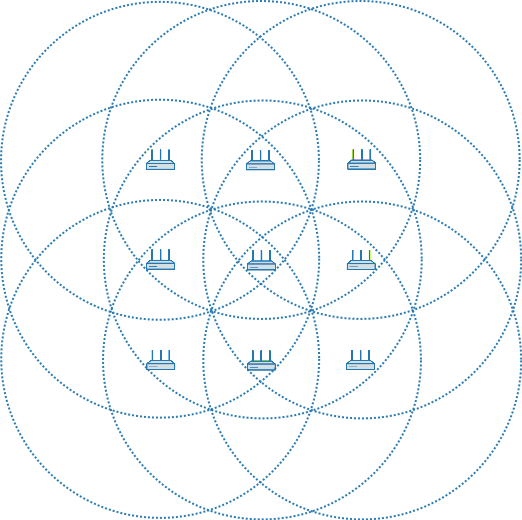
\includegraphics[width=0.41\columnwidth]{figures/3x3ap_range}
      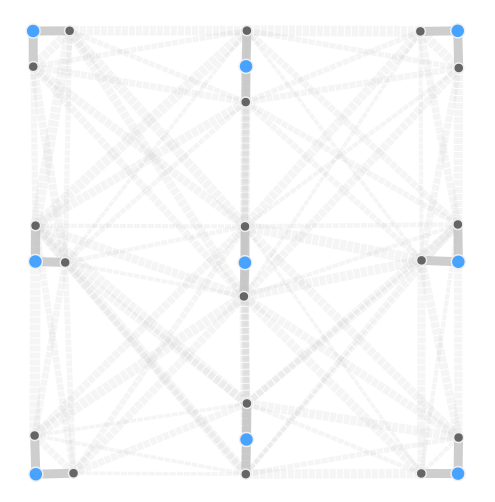
\includegraphics[width=0.41\columnwidth]{figures/bsp_algo/seen}
      \caption{Grid layout with two radio modules per \ac{AP} (left). Resulting network topology (right). Thicker edges indicate higher link-SNR.}
      \label{fig:3x3initial}
    \end{figure}
    
    \begin{figure}[h!]
      \centering
      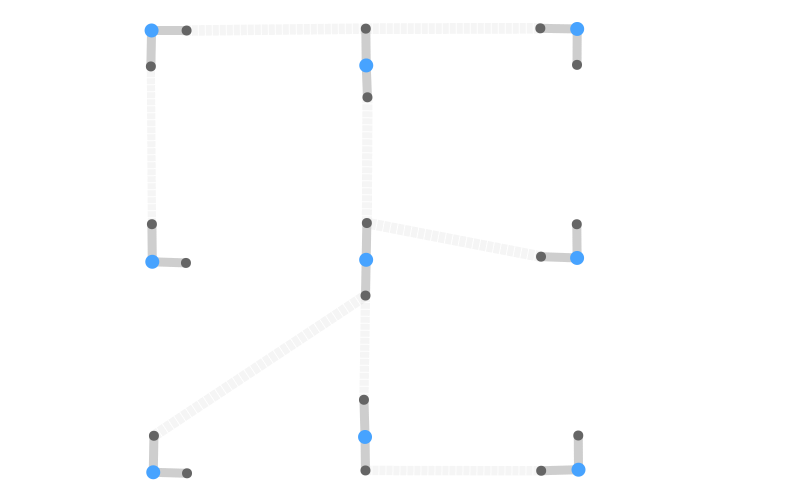
\includegraphics[width=0.41\columnwidth]{figures/bsp_algo/mst}
      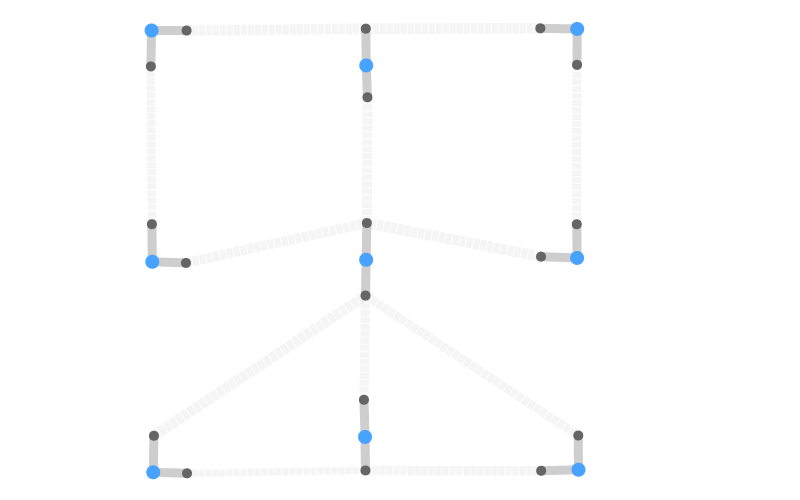
\includegraphics[width=0.41\columnwidth]{figures/bsp_algo/survival}
      \caption{Spanning tree on the graph (left) and spanning tree with survival paths (right)}
      \label{fig:3x3second}
    \end{figure}
    
    \begin{figure}[h!]
      \centering
      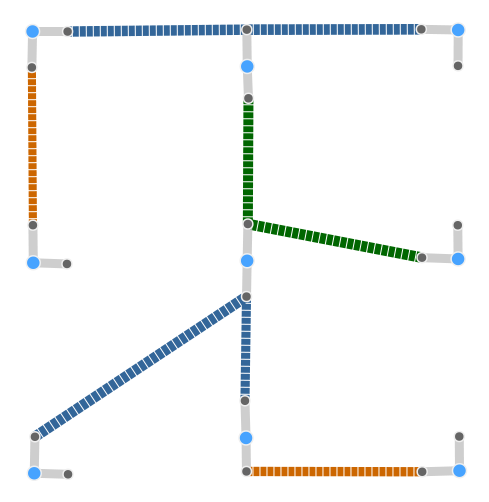
\includegraphics[width=0.41\columnwidth]{figures/bsp_algo/mst_ca}
      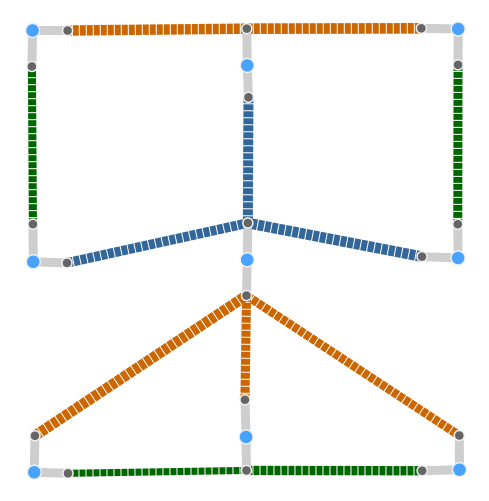
\includegraphics[width=0.41\columnwidth]{figures/bsp_algo/survival_ca}
      \caption{Spanning tree with channels assigned (left) and spanning tree with survival paths with channels assigned (right)}
      \label{fig:3x3third}
    \end{figure}
    
    \newpage
  
  \section{Problems and Aids}
    \begin{description}
    \item [\textit{AutoWDS} Status Tool:]
      To make things easier for debugging and also to actually see what is going on during the execution of the algorithms,
      we created a tool called \textit{AutoWDS} status, which is based on D3.js, a JavaScript library for visualizing data \cite{d3js}.
      Furthermore attached with a tool to extract data from the \ac{WLC}, it is able to display current statuses and established links of a real world, deployed network.
      
      It works by reading a graph represented as a \ac{JSON}-file and displays it interactively in html with JavaScript.
      As it is basically a force directed graph, the nodes position themselves according to their \ac{SNR}-edge-values. 
      Additionally you can drag and position single nodes freely anywhere on the map for better singularization of entities.
      In the tcca module we also included an export function called "write\_json(graph, filename)" which creates a json file to be read by the autowds status tool.
      This tool has also been used to create most of the images in this thesis.

    \item [Representation of Tables in LANCOM Devices:]
      While writing the code which deals with the \ac{WLC} and receives the data, 
      we initially had difficulties extracting the data out of the tables represented in the \ac{WLC} since
      they reside there in a somewhat obscure format and are spread over different tables.
      So that we effectively had to gather the data and join them so that we receive a nice table like Figure \ref{tab:wlc} with which we can work with. 
      Nevertheless we were able to cope with it, although the code for it is somewhat longer and cumbersome.

    \item [Python Logging Module:]
      Another great helper turned out to be the utilization of pythons logger module. 
      We excessively made use of its Error / Warning / Info / Debug statements which made debugging
      a lot easier without being an obstacle if we did not need the output as we could just switch to a different level of logging and enjoy the silence.
    
    \item [Bitbucket:]
      This was another great help in getting things organized.
      Especially git \cite{git} as a version control system and the issue-tracking system one can find in Bitbucket \cite{bitbucket}
      gave us great control and overview on the project without being a hassle to administrate. 
      If you have or want to further work on this project we can only recommend
      getting access to our Bitbucket repository, because there you find additional notes on every issue and basically see why things went the way they did.
      
    \item [PyCharm:]
      For our python coding we used the \ac{IDE} PyCharm \cite{pycharm} and were more than pleased with its speed and debugging possibilities.
      Its refactoring methods made changing the code easy and comfortable.
      Particularly the code analysis tool that comes with it made sticking to the \ac{PEP8} \footnote{See http://legacy.python.org/dev/peps/pep-0008/}
      style-guideline almost fun and we hope it helps you to better understand our code.
      
\newpage
      
    \item [Proof of Concept:]
      We knew from the beginning that a full and complete integration into the existing environment (\ac{LCOS} / \ac{WLC}) was not feasible in the scheduled time frame.
      This is why we aimed at a quick and dirty, proof of concept-like solution which could be easily done with python on a separate machine.
      
    \end{description}

    \begin{figure}[h]
      \centering
      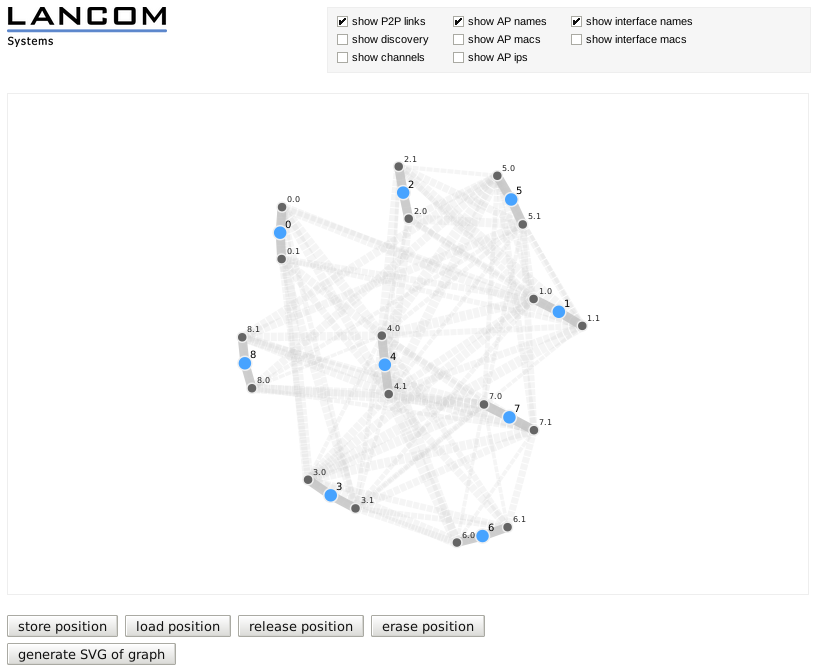
\includegraphics[width=\columnwidth]{figures/autowdsstatus}
      \caption{\textit{AutoWDS} status web interface showing a network topology}
      \label{fig:autowdsstatus}
    \end{figure}
    
\clearpage